\level{1}{Resoconto delle varie attività di verifica - Fase P}
	Sono riportati in questa appendice tutti i risultati ottenuti nei momenti di verifica, stabiliti nel \insdoc{Piano di Progetto v4.00} secondo la strategia di misurazione per il perseguimento della qualità individuata nel presente documento. Ove fosse necessario, sono state tratte anche delle conclusioni sui risultati ottenuti e su come essi possano essere migliorati.
	\level{2}{Verifica dei prodotti}
		\level{3}{Documenti}
			In questa sezione vengono riportati i risultati delle attività di verifica svolte sui documenti. Esse sono di due tipi:
			\begin{itemize}
				\item verifiche manuali;
				\item verifiche automatizzate.
			\end{itemize}
			\level{4}{Verifiche manuali}
				Le attività di verifica manuale della documentazione prodotta sono state svolte in base alla \insglo{procedura} riguardante la verifica dei documenti che è descritta nel documento \insdoc{Norme di Progetto v4.00}.\\
				La verifica manuale ha permesso di individuare soprattutto errori riguardanti le seguenti tipologie:
				\begin{itemize}
					\item descrizioni imprecise di classi e metodi;
					\item errori concettuali;
					\item errori nell'utilizzo della lingua inglese.
				\end{itemize}
				Si riporta di seguito la quantità degli errori rilevati e risolti, per ciascuna tipologia, durante l'intera \insglo{fase}.
				\begin{table}[H]
					\centering
						\begin{tabu}{| l | c |}
							\hline
								Descrizioni imprecise	&	20\\ \hline
								Errori concettuali	&	13\\ \hline
								Errori di inglese  &  34\\ \hline
						\end{tabu}
						\caption{Errori trovati tramite verifica manuale dei documenti durante la Fase P}
				\end{table}
				La verifica manuale dei diagrammi \insglo{UML}, effettuata per controllare la correttezza dei metodi e dei campi dati inseriti per procedere con la stesura della \insdoc{Definizione di Prodotto v1.00}, è risultata piuttosto onerosa, ma poco produttiva, in quanto i \insrole{Progettisti} hanno posto molta attenzione nell'attività di progettazione di dettaglio.\\
				Si può inoltre notare come gli errori concettuali che sono stati trovati siano in leggera diminuzione, segno del fatto che i documenti si stanno piano piano avvicinando al loro contenuto ottimale.\\
				Si noti invece come vi sia una notevole quantità di errori nell'uso della lingua inglese, che nelle altre fasi non c'erano. Questo è dovuto al fatto che è stata cominciata la stesura del manuale, ed esso è scritto in lingua inglese.
			\level{4}{Verifiche automatizzate}
				Le attività di verifica automatizzate sono state effettuate secondo le procedure e attraverso gli strumenti descritti nel documento \insdoc{Norme di Progetto v4.00}. Esse hanno permesso di rilevare diversi errori riguardanti le seguenti tipologie:
				\begin{itemize}
					\item ortografia errata;
					\item utilizzo errato dei comandi \LaTeX{} indicati nelle \insdoc{Norme di Progetto v4.00};
					\item norme tipografiche non rispettate.
				\end{itemize}
				Di seguito è presentato un riassunto della quantità di errori trovati (e successivamente risolti) utilizzando la verifica automatica.
				\begin{table}[H]
					\centering
						\begin{tabu}{| l | c |}
							\hline
							Errori ortografici	& 78	\\ \hline
							Utilizzo errato \LaTeX{}	& 2	\\ \hline
							Errori riguardanti norme tipografiche	& 12	\\ \hline
						\end{tabu}
					\caption{Errori trovati tramite verifica automatica dei documenti durante la Fase P}
				\end{table}
				Come si può notare, gli errori ortografici sono diminuiti rispetto alla \insglo{fase} precedente. Tuttavia, questo è anche imputabile alla minor mole di documentazione che è stata prodotta durante questa \insglo{fase}.\\
				Per quanto riguarda le altre due tipologie di errori, si può notare una certa stabilità rispetto alla \insglo{fase} precedente.\\
				Si riportano i risultati delle misurazioni dell'indice di leggibilità Gulpease relative ai documenti modificati in questa \insglo{fase}.
				\begin{table}[H]
					\centering
						\begin{tabu}{| l | c | c |}
							\hline
							Documenti 							& Gulpease	& Esito		\\ \hline \hline
							Piano di progetto v4.00				& 89 		& Superato  \\ \hline
							Specifica tecnica v1.00				& 68		& Superato \\ \hline
							Norme di Progetto v4.00 			& 68		& Superato  \\ \hline
							Piano di Qualifica v4.00 			& 74		& Superato  \\ \hline
							Definizione di prodotto v1.00		& 84		& Superato \\ \hline
							Glossario v4.00					 	& 68 		& Superato  \\ \hline
						\end{tabu}
					\caption{Esiti del calcolo dell'indice di leggibilità effettuato tramite strumenti automatici durante la Fase P}
				\end{table}
				Si noti che non è stato calcolato l'\insglo{indice Gulpease} relativo al \insdoc{Manuale Utente v1.00} in quanto esso è scritto in lingua inglese e tale indice è relativo alla sola lingua italiana.
		\level{3}{Codice}

			In questa sezione sono riportate, per le parti del progetto implementate in questa prima fase di codifica, i risultati delle metriche calcolate nei momenti di verifica.

		
		\level{4}{Numero di requisiti funzionali obbligatori realizzati}

Si riportano di seguito le percentuali di requisiti funzionali realizzati dalle componenti di \insglo{Norris}.
\begin{table}[H]
	\centering
		\begin{tabu}{| l | c | c |}
			\hline
			Componente	& Percentuale requisiti funzionali obbligatori soddisfatti	& Esito		\\ \hline \hline
			InternalAPIManager	& 90\% 	& Accettabile  \\ \hline
			ExternalAPIManager  & 	93\%	& Ottimale  \\ \hline
			DataModel  & 	89\%	& Accettabile  \\ \hline
		\end{tabu}
	\caption{Esiti del calcolo delle percentuali di requisiti funzionali obbligatori realizzati da Norris durante la Fase P}
\end{table}
<<<<<<< Updated upstream

Si riportano di seguito le percentuali di requisiti funzionali realizzati dalle componenti di \insglo{Chuck}.
=======
Come è possibile notare dalla tabella la percentuale dei requisiti funzionali obbligatori soddisfatti da Norris ha raggiunto un esito generalmente accettabile. 
\\ \\
Si riportano di seguito le percentuali di requisiti funzionali realizzati dalle componenti di Chuck.
>>>>>>> Stashed changes
\begin{table}[H]
	\centering
		\begin{tabu}{| l | c | c |}
			\hline
			Componente	& Numero requisiti funzionali obbligatori soddisfatti	& Esito		\\ \hline \hline
			Directive	& 82\% 	& Accettabile  \\ \hline
			ChartView  & 	93\%	& Ottimale  \\ \hline
			ViewModel  & 	85\%	& Accettabile  \\ \hline
			DataModel  & 	95\%	& Ottimale  \\ \hline
		\end{tabu}
	\caption{Esiti del calcolo delle percentuali di requisiti funzionali obbligatori realizzati da Chuck durante la Fase P}
\end{table}
Come è possibile notare dalla tabella la percentuale dei requisiti funzionali obbligatori soddisfatti da Chuck ha raggiunto un esito generalmente accettabile.

\level{4}{Numeri di parametri di un metodo}
Si riportano di seguito le percentuali dei metodi di Norris e \insglo{Chuck} per numero di parametri.
\begin{table}[H]
	\centering
		\begin{tabu}{| l | c | c | c | c | c |}
			\hline
			Componente	& 0 parametri & 1 parametro & 2 parametri & 3 parametri & Esito		\\ \hline \hline
			\insglo{Norris}	& 41\% & 37\% & 20\% & 2\%	& Superato  \\ \hline
			\insglo{Chuck}  & 55\% & 10\% & 18\% & 2\%	& Superato  \\ \hline
		\end{tabu}
	\caption{Esiti del calcolo della percentuale di metodi per numero di parametri}
\end{table}


\level{2}{Verifica dei processi}

\level{3}{Processo di documentazione}
\level{4}{Livello CMM}
Nonostante i progressi fatti nella capacità di gestione dei processi da parte del gruppo, non è ancora possibile affermare di essere 
giunti al quarto livello \insglo{CMM}, poiché non è ancora in grado di gestire appieno le misurazioni in un'ottica di miglioramento
del processo.
\level{4}{Schedule Variance}
Tutte le attività pianificate nel \insdoc{Piano di Progetto v4.00} sono state svolte rispettando le scadenze; lievi ritardi si sono verificato 
solo nella redazione del \insdoc{Manuale Utente v1.00}, a causa di impegni universitari dei membri del \insglo{team} preposti alla sua stesura, e della 
\insdoc{Definizione di Prodotto v1.00}, per delle indecisioni dei \insrole{progettisti} su come affrontare alcune questioni. Tali ritardi sono 
comunque accettabili e sono stati compensati da una maggiore velocità di svolgimento di altre attività.
Riportiamo di seguito i valori ottenuti calcolando la Schedule Variance sui tempi di stesura di ogni documento:
			\begin{table}[H]
					\centering
					\begin{tabu}{| l | c | c |}
							\hline
							Documenti 							& Schedule Variance	& Esito		\\ \hline \hline
							
							Piano di progetto v4.00				& 2\% 		& Ottimale  \\ \hline
							Norme di Progetto v4.00 			& 3\%		& Ottimale  \\ \hline
							Piano di Qualifica v4.00 			& 1\%		& Ottimale  \\ \hline
							Specifica Tecnica v2.00 			& 1\%		& Ottimali  \\ \hline
							Manuale Utente v1.00 			& -3\%		& Accettabile  \\ \hline
							Definizione di \insglo{Prodotto} v1.00 			& -2\%		& Accettabile  \\ \hline
							Glossario v4.00					 	& 0\% 		& Ottimale  \\ \hline
							Totale processo di documentazione & 2\% & Ottimale \\ \hline
						\end{tabu}
					\caption{Esiti del calcolo della Schedule Variance durante la Fase P}
				\end{table}
\level{4}{Budget Variance}
Le risorse impiegate nella stesura della \insdoc{Definizione di Prodotto v1.00} hanno ecceduto leggermente rispetto alle stime fatte, tuttavia sono state ampiamente coperte 
da quelle previste per l'incremento degli altri documenti che, al contrario, sono risultate sovrabbondanti.
Riportiamo di seguito i valori ottenuti calcolando la Budget Variance sulle risorse utilizzate per la stesura di ogni documento:
			\begin{table}[H]
					\centering
					\begin{tabu}{| l | c | c |}
							\hline
							Documenti 							& Budget Variance	& Esito		\\ \hline \hline
							
							Piano di progetto v4.00				& 0\% 		& Ottimale  \\ \hline
							Norme di Progetto v4.00 			& 3\%		& Ottimale  \\ \hline
							Piano di Qualifica v4.00 			& 1\%		& Ottimale  \\ \hline
							Specifica Tecnica v2.00 			& 2\%		& Ottimale  \\ \hline
							Manuale Utente  			& 0\%		& Ottimale  \\ \hline
							Definizione di \insglo{Prodotto} v1.00 			& -2\%		& Accettabile  \\ \hline
							Glossario v4.00					 	& 0\% 		& Ottimale  \\ \hline
							Totale processo di documentazione & 4\% & Ottimale \\ \hline
						\end{tabu}
					\caption{Esiti del calcolo della Budget Variance durante la Fase P}
				\end{table}
\level{4}{Produttività}
Utilizzando la formula descritta all'interno del presente documento (sezione \nameref{sec:metriche}) è stata calcolata la produttività del processo di documentazione. Questo indice è stato calcolato durante tutti i momenti di verifica previsti dal \insdoc{Piano di Progetto v4.00} per la \insphase{Fase P}, e ciò è stato fatto per ogni documento che è stato redatto nel periodo antecedente la verifica. Ogni documento è stato sottoposto al processo di verifica al più cinque volte. Il calcolo fatto di volta in volta sullo stesso documento tiene conto solo delle nuove sezioni introdotte in esso.\\
Segue un riassunto di quanto è stato fatto.
\begin{table}[H]
      \centering
		\begin{tabu}{| l | c | c | c | c | c |}
		\hline
<<<<<<< Updated upstream
		&1	&2	&3	&4	&5	\\ \hline
		Norme di Progetto	& 173 &	&	&	& \\ \hline
		Piano di Progetto	& 170 &	&	&	& \\ \hline
		Piano di Qualifica	& 253	&	&	&	&\\ \hline
		Definizione di \insglo{Prodotto} & 156 &	 	&	&  	&\\ \hline
		Manuale Utente & 143	&	&	&	& \\ \hline
		Glossario & 120 &  & & &\\ \hline
=======
		&1	&2	\\ \hline
		Norme di Progetto	& 173 &	 \\ \hline
		Piano di Progetto	& 170 &	 \\ \hline
		Piano di Qualifica	& 253 & \\ \hline
		Definizione di Prodotto & 156 & 140	 \\ \hline
		Manuale Utente & 143 &   \\ \hline
		Glossario & 120 &  \\ \hline
>>>>>>> Stashed changes
		\end{tabu}
		\caption{Produttività delle varie attività del processo di documentazione durante la fase P}
\end{table}
Di seguito vengono riportati in un grafico i valori della produttività del processo di documentazione rilevati nei vari periodi della \insphase{Fase P} nei quali è stato applicato il processo di verifica. Il grafico fa riferimento alla tabella precedente.\\
\begin{figure}[H]
	\centering
		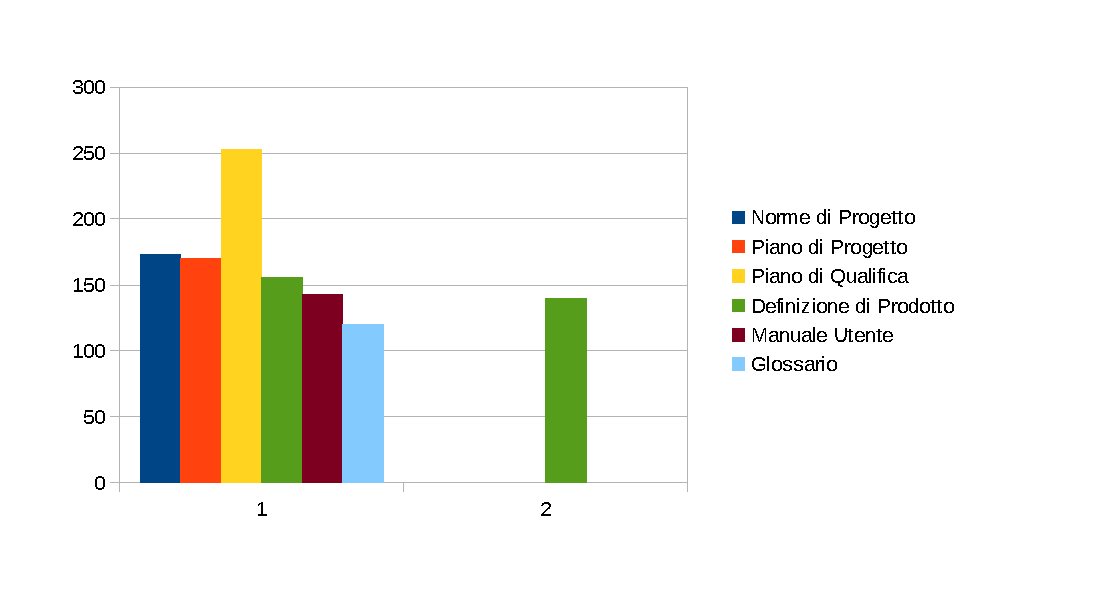
\includegraphics[width=12cm]{PianoDiQualifica/Pics/ProduttivitaDocumentazioneFaseP.pdf}
	\caption{Produttività del processo di documentazione durante la Fase P}
\end{figure}
L'alta produttività dei documenti che hanno subito un incremento deriva dal fatto che le nuove parti aggiunte, seppur ampie, hanno richiesto solo una modesta quantità di risorse.
Al contrario, i livelli di produttività della \insdoc{Definizione di Prodotto v1.00} e del \insdoc{Manuale Utente} risultano leggermente più bassi in quanto la stesura della loro prima versione ha richiesto maggior tempo.

\level{3}{Processo di verifica}
\level{4}{Livello CMM}
	Nonostante l'adozione di nuove metriche e una maggiore regolamentazione del processo di verifica, il \insglo{team} non è ancora in grado di individuare miglioramenti tali da comportare un oggettivo aumento della capacità di gestione del processo, necessario per raggiungere il quarto livello \insglo{CMM}, pertanto il processo di verifica rimane al terzo livello (Definito).
\level{4}{Schedule Variance}
	Il processo di verifica è stato sempre svolto rispettando le scadenze temporali previste nel \insdoc{Piano di Progetto v4.00}. I valori della Schedule Variance calcolati per questo processo risultano quindi ottimi.\\
			Riportiamo di seguito il valore ottenuti:
			\begin{table}[H]
				\centering
				\begin{tabu}{| l | c | c |}
					\hline
						Processi 							& Schedule Variance	& Esito		\\ \hline \hline
						Processo di verifica & 0\% & Ottimale \\ \hline
				\end{tabu}
				\caption{Esiti del calcolo della Schedule Variance durante la Fase P}
			\end{table}	

\level{4}{Budget Variance}
Le risorse utilizzate nel processo di verifica sono risultate in linea con le stime del \insdoc{Piano di Progetto v4.00}, risultando anche leggermente sovrastimate.
Riportiamo di seguito il valore ottenuti:
\begin{table}[H]
	\centering
	\begin{tabu}{| l | c | c |}
	\hline
	Processi 							& Budget Variance	& Esito		\\ \hline \hline
	Processo di verifica & 1\% & Ottimale \\ \hline
	\end{tabu}
	\caption{Esiti del calcolo della Budget Variance durante la Fase P}
\end{table}	

\level{4}{Produttività}
Utilizzando la formula descritta all'interno del presente documento (sezione \nameref{sec:metriche}) è stata calcolata la produttività del processo di verifica. Tale indice è stato calcolato in seguito a tutti i momenti di verifica previsti dal \insdoc{Piano di Progetto v4.00} per la \insphase{Fase P}. Di seguito vengono riportati i valori calcolati e una loro rappresentazione grafica.
\begin{table}[H]
	\centering
	\begin{tabu}{| c | c |}
		\hline
		Data verifica &Produttività\\ \hline \hline
		06/04 & 6 \\ \hline
		07/04 & 10 \\ \hline
		09/04 & 3 \\ \hline
		12-14/04 & 3 \\ \hline
		15/04 & 15 \\ \hline
		18/04 & 8 \\ \hline							
	\end{tabu}
	\caption{Produttività del processo di verifica durante la fase P}
\end{table}
\begin{figure}[H]
	\centering
	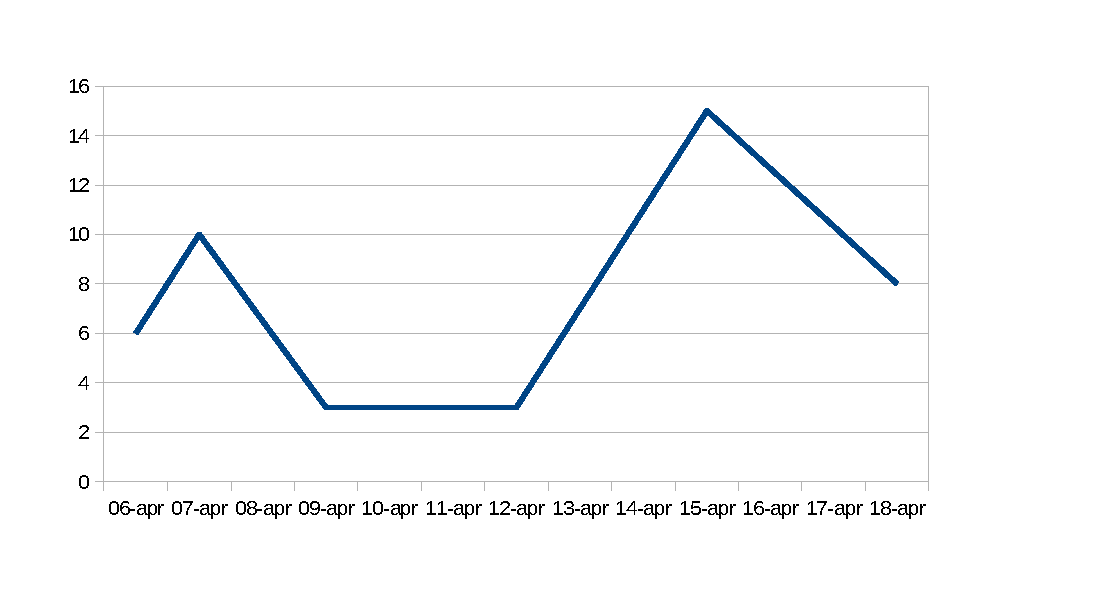
\includegraphics[width=12cm]{PianoDiQualifica/Pics/ProduttivitaVerificaFaseP.pdf}
	\caption{Produttività del processo di verifica durante la Fase P}
\end{figure}
Si può notare che la produttività delle attività di verifica è in media più bassa rispetto alla Fase SD. Ciò è dovuto ad una notevole diminuzione delle anomalie all’interno dei documenti a cui sono stati apportati incrementi. Sono presenti dei picchi in corrispondenza delle verifiche al documento \insdoc{Definizione di Prodotto v1.00}. Ciò è probabilmente dovuto al fatto che questa è la prima esperienza di progettazione software in dettaglio per tutti i membri del team, dunque il numero di errori riscontrati durante l’attività di verifica è elevato.

\level{4}{Efficacia di una revisione}
Utilizzando la formula descritta all'interno del presente documento (sezione \nameref{sec:metriche}) è stata calcolata l'efficacia delle varie revisioni che sono state fatte durante la \insphase{Fase P}. Di seguito vengono riportati i valori calcolati e una loro rappresentazione grafica.
\begin{table}[H]
	\centering
	\begin{tabu}{| c | c |}
	\hline
	Data verifica &Efficacia\\ \hline \hline
	06/04 & 7 \\ \hline
	07/04 & 9 \\ \hline
	09/04 & 2 \\ \hline
	12-14/04 & 0.2 \\ \hline
	15/04 & 0.8 \\ \hline
	18/04 & 6 \\ \hline				
	\end{tabu}
	\caption{Efficacia delle revisioni durante la fase P}
\end{table}
\begin{figure}[H]
	\centering
	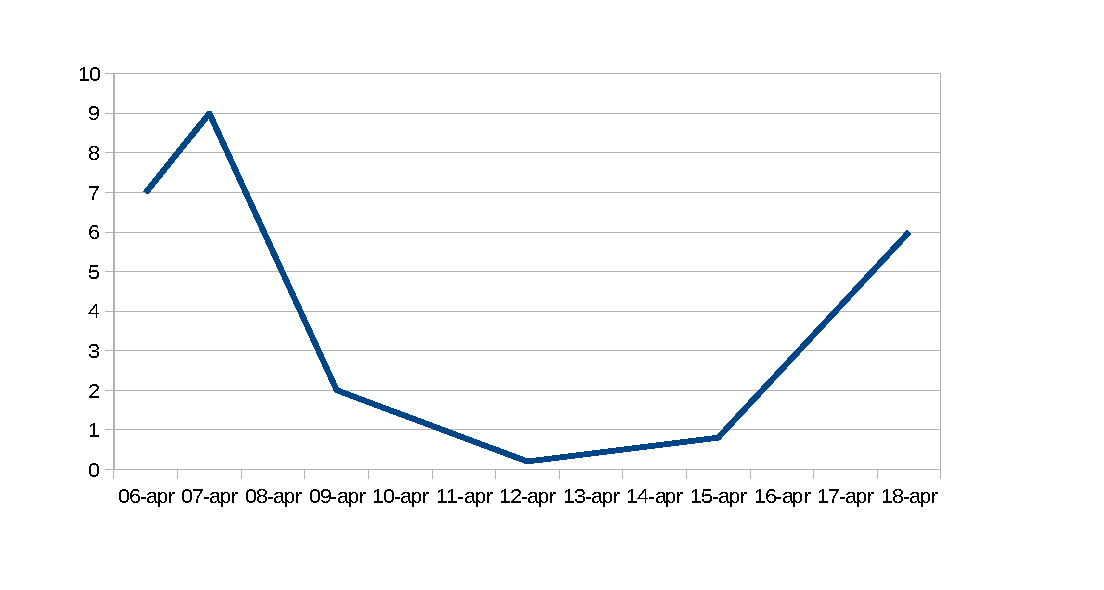
\includegraphics[width=12cm]{PianoDiQualifica/Pics/EfficaciaRevisioniFaseP.pdf}
	\caption{Efficacia delle revisioni durante la Fase P}
\end{figure}
I valori delle due metriche di processo sopra riportate devono essere letti considerando che:
\begin{itemize}
	\item il 6 aprile è stato in gran parte dedicato alle verifiche sugli incrementi apportati ai documenti precedentemente redatti;
	\item il 7 aprile è stata verificata la \insdoc{Definizione di Prodotto v1.00}, riscontrando diversi errori, vista la sua prima stesura, e impiegando una discreta quantità di tempo;
	\item le verifiche avvenute nei giorni 12, 13, 14 e 15 aprile hanno avuto per oggetto codice sorgente e non documenti, pertanto il rapporto viene fatto su righe di codice esaminate, risultando così molto basso;
	\item il 18 aprile si è proceduto a verificare il \insdoc{Manuale utente}, anch'esso alla prima versione, riscontrando diversi errori.
\end{itemize}

\level{3}{Processo di sviluppo}
Si riportano in questa sezione gli esiti delle misurazioni effettuate rispetto all'attività di codifica.
\level{4}{Livello CMM}
Il livello \insglo{CMM} identificato dal \groupname{} per l'attività di codifica è il due, in quanto è stato condotta in maniera normata, facendo attenzione a porre sotto documentazione le scelte progettuali prese e fornendo una discreta documentazione relativa ai prodotti realizzati. Il processo di sviluppo, rispetto a tale attività, risulta infatti disciplinato e ripetibile.
\level{4}{Schedule Variance}
Tutte le attività di codifica sono state svolte secondo le tempistiche programmate nel \insdoc{Piano di Progetto v4.00}.\\

Riportiamo di seguito i valori ottenuti calcolando la Schedule Variance sui tempi di stesura del codice sorgente.
			\begin{table}[H]
				\centering
				\begin{tabu}{| l | c | c |}
					\hline
						Processi 							& Schedule Variance	& Esito		\\ \hline \hline
						Processo di sviluppo (codifica) & 0\% & Ottimale \\ \hline
				\end{tabu}
				\caption{Esiti del calcolo della Schedule Variance durante la Fase P}
			\end{table}	
			
\level{4}{Budget Variance}
Le risorse previste per l'attività di codifica in questa \insglo{fase} sono risultate leggermente sovrastimate, in quanto i codici sorgenti della libreria grafica \insglo{Chuck} sono molto simili, in alcune loro parti, a quelle del \textit{\insglo{framework}} \insglo{Norris}.
			\begin{table}[H]
				\centering
				\begin{tabu}{| l | c | c |}
					\hline
						Processi 							& Budget Variance	& Esito		\\ \hline \hline
						Processo di sviluppo (codifica) & 1\% & Ottimale \\ \hline
				\end{tabu}
				\caption{Esiti del calcolo della Budget Variance dell'attività di codifica durante la Fase P}
			\end{table}	
\level{4}{Produttività}
Utilizzando la formula descritta all'interno del presente documento (sezione \nameref{sec:metriche}) è stata calcolata la produttività del processo di sviluppo, limitatamente all'attività di codifica. Questo indice è stato calcolato durante i due momenti di verifica previsti dal \insdoc{Piano di Progetto v4.00} per la \insphase{Fase P}.\\
Seguono i risultati delle misurazioni.
\\\begin{table}[H]
				\centering
				\begin{tabu}{| l | c | c |}
					\hline
						Processi 							& 1	& 2		\\ \hline \hline
						Processo di sviluppo (codifica) & 33 & 29  \\ \hline
				\end{tabu}
				\caption{Esiti del calcolo della produttività della codifica durante la Fase P}
			\end{table}	

\level{3}{PDCA}
In questa sezione viene riportato il grafico \insglo{PDCA} della \insphase{Fase P}. In ascissa è rappresentato il tempo, in ordinata le attività.
\begin{figure}[H]
	\centering
	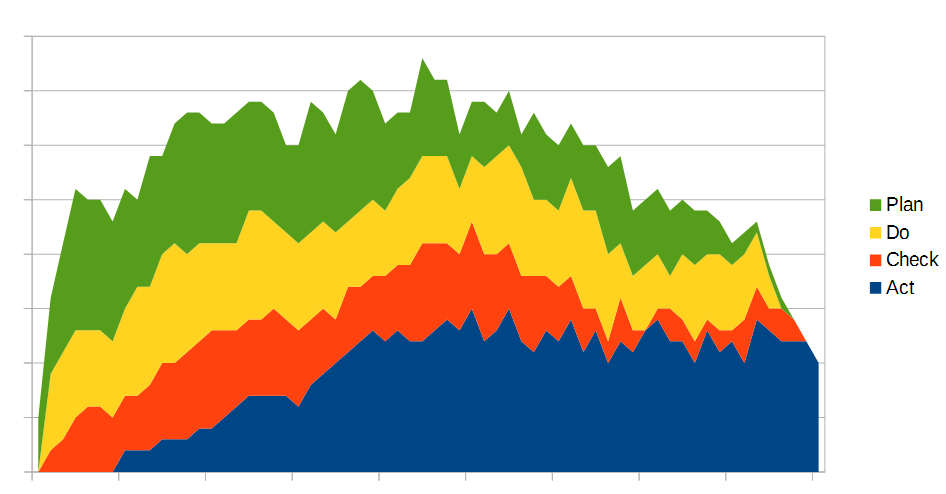
\includegraphics[width=0.6\textwidth]{PianoDiQualifica/Pics/GraficoPDCAFaseP.png}
	\caption{PDCA Fase P}
\end{figure}
Guardando il primo terzo del grafico è facilmente intuibile il fatto che le attività pianificate siano state difficili da consumare mettendo subito in allerta il \insrole{Responsabile di Progetto}. Infine è possibile notare come nei rimanenti due terzi di grafico la situazione sia andata decisamente meglio portando il grafico a convergere. Tale fatto è imputabile sicuramente al lavoro fatto dal \insrole{Project Manager} durante la pianificazione. Infatti gli slack non utilizzati aggiunti nelle attività della seconda parte di grafico hanno permesso di colmare l'iniziale dilungamento subito.